%
%

%%-----------------------------------------------------
%%-----------------------------------------------------
\section{Coffeescript}

%%-----------------------------------------------------
\begin{frame}
\frametitle{The basics}

\begin{columns}[T]
\begin{column}{.48\textwidth}
\begin{center}

\includegraphics[width=3.5cm]{figs/coffeescript}
\end{center}
\begin{flushright}
  {\Large
    \url{coffeescript.org}
  }
\end{flushright}

\end{column}%
\hfill%
\begin{column}{.50\textwidth}
{\Large
\begin{itemize}
  \item Sintaxis más sencilla
  \item Orientado a ser legible
  \item Breve
  \item Indentación
  \item No hay paréntesis
  \item En 2012 fue el 11º lenguage más popular en GitHub
  \item Se puede probar en línea
\end{itemize}
}
\end{column}%
\end{columns}

\end{frame}

%%-----------------------------------------------------
\begin{frame}
\frametitle{¿Cómo funciona?}

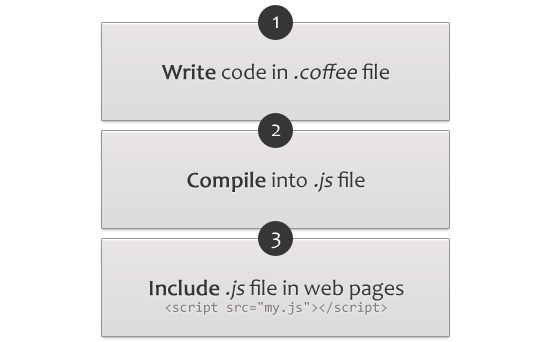
\includegraphics[width=11.5cm]{figs/coffeescript_works.jpg} 
% Imagen sacada de http://sixrevisions.com/javascript/coffeescript-basics/

\end{frame}

%%-----------------------------------------------------
\begin{frame}
\frametitle{Ejemplos}

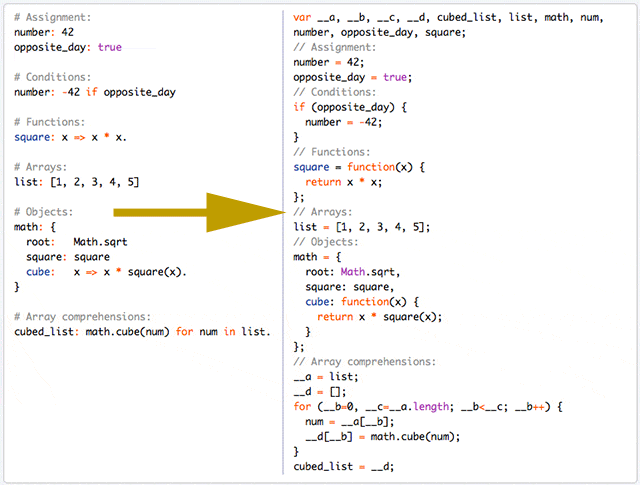
\includegraphics[width=11.5cm]{figs/coffeescript_example.png} 
% Imagen sacada de http://www.rubyinside.com/rails-3-1-adopts-coffeescript-jquery-sass-and-controversy-4669.html


\end{frame}






